\documentclass[../../Problems]{subfiles}
\begin{document}
\KOMAoptions{paper=A3}
\recalctypearea
\subsection{Chaos Game (Iterated Function Systems)}
Intuitively, in these systems, we iterate a specific function repeatedly. For simplicity, let us only consider affine transformations\footnote{In general, affine transformations are of the form $Ax+b$ where $A$ is a matrix and $x,b$ are vectors.}. We take a random initial point $P=\begin{bmatrix}x\\y\end{bmatrix}$ and repeatedly apply different affine transformations to get $P_{\text{next}}=f_i(P)$ with some probability $p_i$. After large number of iterations, a pattern emerges!
\begin{equation}
	f(x,y)={\begin{bmatrix}a&b\\c&d\end{bmatrix}}{\begin{bmatrix}x\\y\end{bmatrix}}+{\begin{bmatrix}e\\f\end{bmatrix}}
\end{equation}
\begin{note}
	You can get probabilities by smartly generating random numbers. \verb!randuv(x, y)! (Simplecpp library) generates random numbers (\verb!double!) between $x$ and $y$. If you feel adventurous then implement your own random number generator using \hyperref[pp:linearfeedbackshiftregister]{LFSRs} :).
\end{note}
% \vspace{-2em}
\subsubsection{Sierpi\'nski Triangle}{\label{pp:sierpinskitriangle}}
Consider $A,B,C$ as some co-ordinates of an equilateral triangle. Now, after taking a random initial point $P$ we go half the distance towards $A$ or $B$ or $C$ with equal probability and repeat this with the new point over and over. This operation can be representated using affine transformations as below
\begin{align}
	\text{With probability 1/3, apply }& \quad f_{1}(x,y) = {\begin{bmatrix}0.05&0.00\\0.00&0.05\end{bmatrix}}{\begin{bmatrix}x\\y\end{bmatrix}}+\frac{1}{2}{\begin{bmatrix}A_x \\ A_y \end{bmatrix}}\\
	\text{With probability 1/3, apply }& \quad f_{2}(x,y) = {\begin{bmatrix}0.05&0.00\\0.00&0.05\end{bmatrix}}{\begin{bmatrix}x\\y\end{bmatrix}}+\frac{1}{2}{\begin{bmatrix}B_x \\ B_y \end{bmatrix}}\\
	\text{With probability 1/3, apply }& \quad f_{3}(x,y) = {\begin{bmatrix}0.05&0.00\\0.00&0.05\end{bmatrix}}{\begin{bmatrix}x\\y\end{bmatrix}}+\frac{1}{2}{\begin{bmatrix}C_x \\ C_y \end{bmatrix}}
\end{align}
In limit, we get the Sierpi\'nski Triangle.

\textbf{Problem Statement:}\\
Simulate this system and observe the generated pattern using \verb!turtleSim! with appropriate scaling such that it takes same width and height for all iterates.
\begin{tcolorbox}[breakable, enhanced, sharpish corners]%, colback = white]
	\href{https://github.com/paramrathour/CS-101/blob/main/Starter%20Codes/Sierpi%C5%84ski%20Triangle.cpp}{\textbf{Starter Code}}
\end{tcolorbox}
\begin{figure}[H]
	\centering
	\begin{subfigure}{0.18\linewidth}
		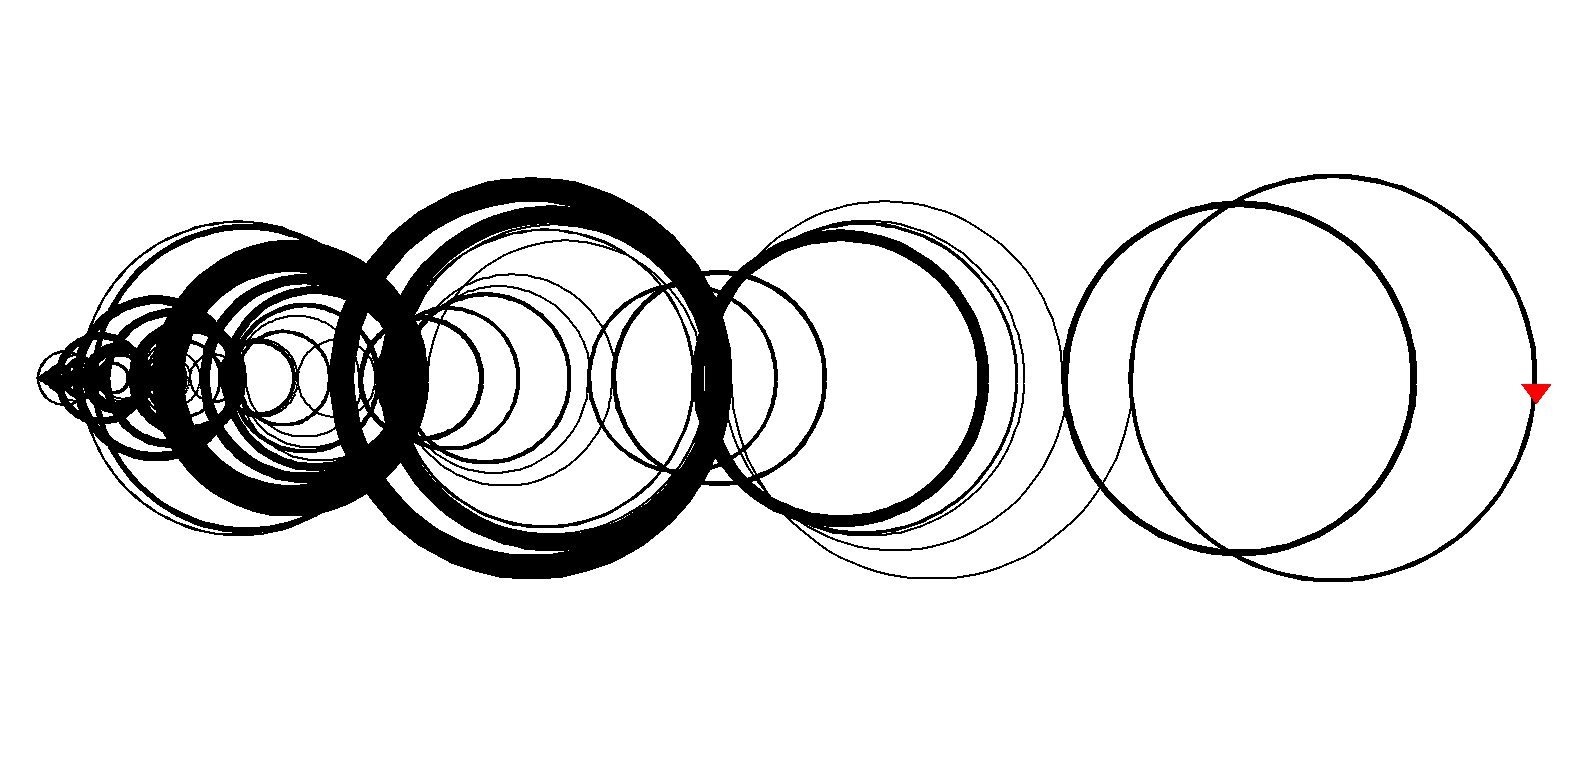
\includegraphics[width = \linewidth]{Sierpiński Triangle/10.png}
		\caption{Iterate 10}
	\end{subfigure}
	\begin{subfigure}{0.18\linewidth}
		\includegraphics[width = \linewidth]{Sierpiński Triangle/100.png}
		\caption{Iterate 100}
	\end{subfigure}
	\begin{subfigure}{0.18\linewidth}
		\includegraphics[width = \linewidth]{Sierpiński Triangle/1000.png}
		\caption{Iterate 1000}
	\end{subfigure}
	\begin{subfigure}{0.18\linewidth}
		\includegraphics[width = \linewidth]{Sierpiński Triangle/10000.png}
		\caption{Iterate 10000}
	\end{subfigure}
	\begin{subfigure}{0.18\linewidth}
		\includegraphics[width = \linewidth]{Sierpiński Triangle/100000.png}
		\caption{Iterate 100000}
	\end{subfigure}
	\caption{Sierpi\'nski Triangle for iterates growing with power of 10}
\end{figure}
\vspace{-2em}
\subsubsection{Barnsley's Fern}{\label{pp:barnsleyfern}}
Again, by taking different $f_i$, we get different fractal. An explain
\begin{align}
	\text{With probability 0.01, apply }& \quad f_{1}(x,y) = {\begin{bmatrix}0.00&0.00\\0.00&0.16\end{bmatrix}}{\begin{bmatrix}x\\y\end{bmatrix}}\\
	\text{With probability 0.85, apply }& \quad f_{2}(x,y) = {\begin{bmatrix}0.85&0.04\\-0.04&0.85\end{bmatrix}}{\begin{bmatrix}x\\y\end{bmatrix}}+{\begin{bmatrix}0.00\\1.60\end{bmatrix}}\\
	\text{With probability 0.07, apply }& \quad f_{3}(x,y) = {\begin{bmatrix}0.20&-0.26\\0.23&0.22\end{bmatrix}}{\begin{bmatrix}x\\y\end{bmatrix}}+{\begin{bmatrix}0.00\\1.60\end{bmatrix}}\\
	\text{With probability 0.07, apply }& \quad f_{4}(x,y) = {\begin{bmatrix}-0.15&0.28\\0.26&0.24\end{bmatrix}}{\begin{bmatrix}x\\y\end{bmatrix}}+{\begin{bmatrix}0.00\\0.44\end{bmatrix}}
\end{align}
In limit, we get the Barnsley's Fern.

\textbf{Problem Statement:}\\
Simulate this system and observe the generated pattern using \verb!turtleSim! with appropriate scaling such that it takes same width and height for all iterates.
\begin{tcolorbox}[breakable, enhanced, sharpish corners]%, colback = white]
	\href{https://github.com/paramrathour/CS-101/tree/main/Starter Codes/Barnsley's Fern.cpp}{\textbf{Starter Code}}
\end{tcolorbox}
\begin{figure}[H]
	\centering
	\begin{subfigure}{0.22\linewidth}
		\includegraphics[width = \linewidth]{Barnsley's Fern/100.png}
		\caption{Iterate 100}
	\end{subfigure}
	\begin{subfigure}{0.22\linewidth}
		\includegraphics[width = \linewidth]{Barnsley's Fern/1000.png}
		\caption{Iterate 1000}
	\end{subfigure}
	\begin{subfigure}{0.22\linewidth}
		\includegraphics[width = \linewidth]{Barnsley's Fern/10000.png}
		\caption{Iterate 10000}
	\end{subfigure}
	\begin{subfigure}{0.22\linewidth}
		\includegraphics[width = \linewidth]{Barnsley's Fern/100000.png}
		\caption{Iterate 100000}
	\end{subfigure}
	\caption{Barnsley's Fern for iterates growing with power of 10}
\end{figure}
\begin{funvideo}
	\href{https://youtu.be/kbKtFN71Lfs}{Chaos Game -- Numberphile}\\
	\href{https://youtu.be/IGlGvSXkRGI}{Chaos Game | Fractals emerging from chaos | Computer simulation -- Think Twice}
\end{funvideo}
\KOMAoptions{paper=A4}
\recalctypearea
\end{document}